\documentclass{article}
\usepackage{tikz}

\begin{document}


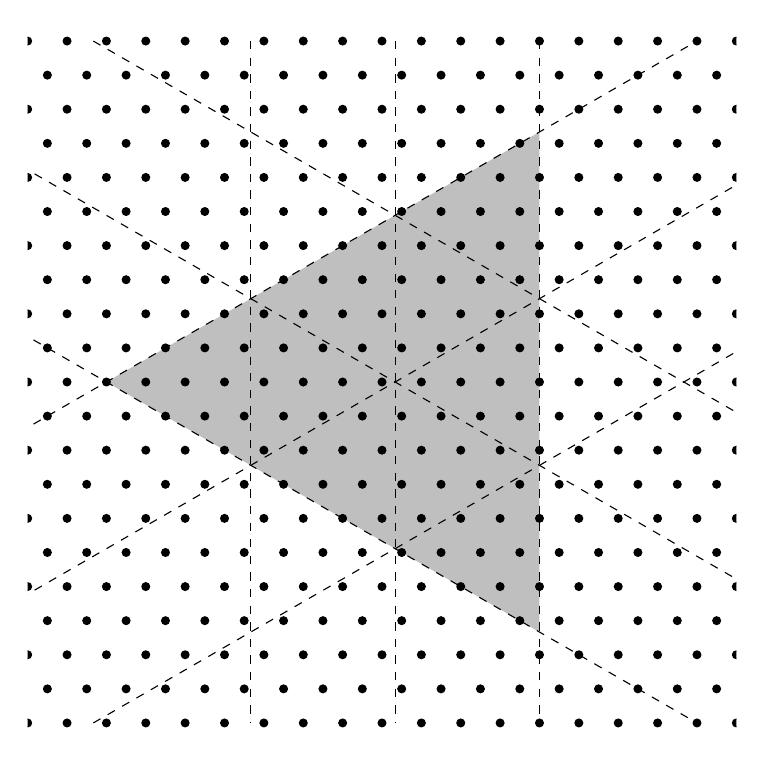
\begin{tikzpicture}[scale=.5]

\begin{scope}
\clip (-9,-9)--(-9,9)--(9,9)--(9,-9)--cycle;

%\clip (-7.3,0)--(4.15, 3.81666*1.7320508)--(4.15, -3.81666*1.7320508)--cycle;
%\clip (-3.5, -4*1.7320508/2)--(-3.5, 4*1.7320508/2)--(2.5,
%4*1.7320508/2)--(2.5, -4*1.7320508/2)--cycle;

\fill[gray!50] (-7,0)--(4, 11/3*1.7320508)--(4, -11/3*1.7320508)--cycle;

\foreach \x in {-14,-13,...,14}{% Two indices running over each
    \foreach \y in {-10,-9,...,10}{% node on the grid we have drawn
        \node[draw,circle,inner sep=1pt,fill] at (\x-\y/2,1.7320508*\y/2) {};}}

\draw[dashed] (1/3, 10*1.7320508/2)--(1/3, -5*1.7320508);
\draw[dashed] (-10/3, 10*1.7320508/2)--(-10/3, -5*1.7320508);

\draw[dashed] (4, 10*1.7320508/2)--(4, -5*1.7320508);
\draw[dashed] (-15-7, 5*1.7320508)--(15-7, -5*1.7320508);
\draw[dashed] (-15+1/3, 5*1.7320508)--(15+1/3, -5*1.7320508);
\draw[dashed] (-15+7+2/3, 5*1.7320508)--(15+7+2/3, -5*1.7320508);

\draw[dashed] (-15-7, -5*1.7320508)--(15-7, 5*1.7320508);
\draw[dashed] (-15+1/3, -5*1.7320508)--(15+1/3, 5*1.7320508);
\draw[dashed] (-15+7+2/3, -5*1.7320508)--(15+7+2/3, 5*1.7320508);

\end{scope}
\end{tikzpicture}



\begin{tikzpicture}[scale=.5]

\foreach \x in {-7,-6,...,7}{% Two indices running over each
    \foreach \y in {-7,-6,...,7}{% node on the grid we have drawn
        \node[draw,circle,inner sep=1pt,fill] at (\x/2, 1.7320508*\x/6+1.7320508*\y/3) {};}}


\draw[dashed] (1/3, 10*1.7320508/2)--(1/3, -5*1.7320508);
\draw[dashed] (-10/3, 10*1.7320508/2)--(-10/3, -5*1.7320508);

\draw[dashed] (4, 10*1.7320508/2)--(4, -5*1.7320508);
\draw[dashed] (-15-7, 5*1.7320508)--(15-7, -5*1.7320508);
\draw[dashed] (-15+1/3, 5*1.7320508)--(15+1/3, -5*1.7320508);
\draw[dashed] (-15+7+2/3, 5*1.7320508)--(15+7+2/3, -5*1.7320508);

\draw[dashed] (-15-7, -5*1.7320508)--(15-7, 5*1.7320508);
\draw[dashed] (-15+1/3, -5*1.7320508)--(15+1/3, 5*1.7320508);
\draw[dashed] (-15+7+2/3, -5*1.7320508)--(15+7+2/3, 5*1.7320508);



\end{tikzpicture}




\end{document}


\begin{scope}[xshift=9cm]
\clip (-3.5, -4*1.7320508/2)--(-3.5, 4*1.7320508/2)--(2.5,
4*1.7320508/2)--(2.5, -4*1.7320508/2)--cycle;

\fill[gray!50] (-3,0)--(2, 5/3*1.7320508)--(2, -5/3*1.7320508)--cycle;
\draw[thick, blue] (.333,0) circle(.08);
\foreach \x in {-7,-6,...,7}{% Two indices running over each
    \foreach \y in {-7,-6,...,7}{% node on the grid we have drawn
        \node[draw,circle,inner sep=1pt,fill] at (\x-\y/2,1.7320508*\y/2) {};}}


\begin{scope}[green, xshift=.5cm, yshift=.2886751cm]
\foreach \x in {-7,-6,...,7}{% Two indices running over each
    \foreach \y in {-7,-6,...,7}{% node on the grid we have drawn
        \node[draw,circle,inner sep=.7pt,fill] at (\x-\y/2,1.7320508*\y/2) {};}}
\end{scope}

\begin{scope}[red, xshift=.5cm, yshift=-.2886751cm]
\foreach \x in {-7,-6,...,7}{% Two indices running over each
    \foreach \y in {-7,-6,...,7}{% node on the grid we have drawn
        \node[draw,circle,inner sep=.7pt,fill] at (\x-\y/2,1.7320508*\y/2) {};}}
\end{scope}

\draw[dashed] (2, 10*1.7320508/2)--(2, -5*1.7320508);
\draw[dashed] (-15-3, 5*1.7320508)--(15-3, -5*1.7320508);
\draw[dashed] (-15-3, -5*1.7320508)--(15-3, 5*1.7320508);
\end{scope}

\end{tikzpicture}

\newpage
\begin{tikzpicture}

\begin{scope}[green, xshift=.5cm, yshift=.2886751cm]
\foreach \x in {0,1,...,7}{% Two indices running over each
    \foreach \y in {0,1,...,7-\x}{% node on the grid we have drawn
        \node[draw,circle,inner sep=.7pt,fill] at (\x-\y/2,1.7320508*\y/2) {};}}
\end{scope}


\end{tikzpicture}


\end{document}
